\begin{figure}[h]
    \centering
    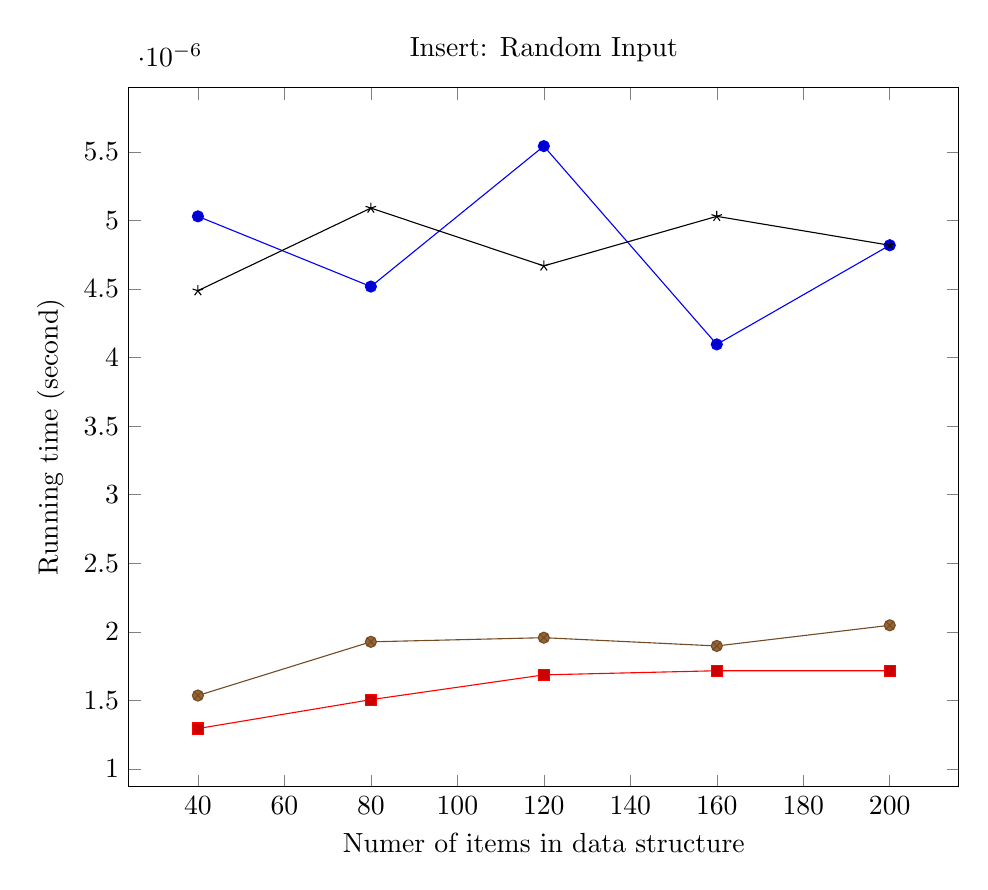
\begin{tikzpicture}
        \begin{axis}[
            xlabel={Numer of items in data structure},
            ylabel={Running time (second)},
            title={Insert: Random Input},
            width=\textwidth
        ]
		\addplot coordinates {
			(40, 5.029628123752461e-06)
			(80, 4.517630051274757e-06)
			(120, 5.541626196230165e-06)
			(160, 4.0959845798216324e-06)
			(200, 4.818805388026593e-06)
		};
		\addplot coordinates {
			(40, 1.2950539480319212e-06)
			(80, 1.5058766837577896e-06)
			(120, 1.686581885808336e-06)
			(160, 1.716699419485046e-06)
			(200, 1.716699419485046e-06)
		};
		\addplot coordinates {
			(40, 1.535994217433112e-06)
			(80, 1.927522155209527e-06)
			(120, 1.9576396888862367e-06)
			(160, 1.8974046215355922e-06)
			(200, 2.0479922899108162e-06)
		};
		\addplot coordinates {
			(40, 4.487512517600823e-06)
			(80, 5.089863191103105e-06)
			(120, 4.668217719651368e-06)
			(160, 5.029628123752461e-06)
			(200, 4.818805388026593e-06)
		};
        \legend{}
        \end{axis}
    \end{tikzpicture}
    \caption{Average of 0 operations, benchmarked every 0, starting at 0.}
\end{figure}